% ===========================================================================
% ASPLOS 2027 (September cycle) submission.
% Template per the CFP: acmart with sigplan, anonymous, review, nonacm.
% 10pt, two-column, US Letter.  No spacing or font manipulation is used.
% ===========================================================================
\documentclass[sigplan,10pt,anonymous,review,nonacm]{acmart}

\settopmatter{printfolios=true,printccs=false,printacmref=false}

% acmart already loads amsmath and the newtx symbol set; loading amssymb here
% redefines \Bbbk and errors out, so it is deliberately absent.
\usepackage{booktabs}
\usepackage{graphicx}
\usepackage{enumitem}
\usepackage{pifont}
% The balance package is deliberately not loaded: it rebalanced the final
% columns past the bottom of the text block, which pushed body text roughly
% 0.8in below the 1in bottom margin on the last appendix page.

% Last-resort inter-word stretch for the narrow two-column measure.  This
% only engages on lines that would otherwise be overfull; it changes no
% vertical spacing and no font size, and it does not fit more content on a
% page.  Without it the long model identifiers and version strings below
% push into the gutter.
\emergencystretch=1.2em

\newcommand{\cmark}{\ding{51}}
\newcommand{\xmark}{\ding{55}}
\newcommand{\Sres}{\mathcal{S}_{\text{res}}}
\newcommand{\Ssys}{\mathcal{S}_{\text{sys}}}
\newcommand{\beff}{b_{\text{eff}}}
\newcommand{\bpt}{\,bits/elem}

% The harness is public under a different name; per the ASPLOS anonymity
% rules ("if your system is already released to the public, rename it in
% your submission") it is referred to throughout by this pseudonym.
\newcommand{\sys}{TriAxis}

\begin{document}

% The optional argument sets the running head. Giving a short running title
% for a long title is ordinary acmart practice; it also stops the odd-page
% running head from spanning the full column, which is what the ASPLOS format
% checker was mistaking for a line of body text above the text block.
\title[Compression Ratio Is Not a Serving Metric]{%
       Compression Ratio Is Not a Serving Metric: A Measurement Study of
       KV-Cache Compression for Long-Context LLM Serving}

\author{Anonymous Author(s)}
\affiliation{\institution{Submission under double-blind review}\country{}}

\begin{abstract}
Long-context LLM serving is bounded by the key--value (KV) cache, and a large
literature compresses it. Almost all of that literature summarises a method to
a prospective adopter with two numbers: a compression ratio and a task score.
A serving system consumes neither; it consumes prefill latency, decode
throughput and resident device memory. We ask whether the two reported numbers
predict the three consumed ones, and measure that in our study they do not.

Across 3{,}150 paired query executions --- each compressed run matched to an
uncompressed run of the same model on the identical prompt --- spanning seven
compression methods, three open-weight models, five long-context tasks and
contexts from 2K to 128K tokens, we find: (i) at an \emph{identical} nominal
budget of 4 bits per KV element, with realised payloads within $0.19$ bits of
one another, task accuracy ranges from $2.5\%$ to $47.3\%$ on one model, an
$18.7\times$ spread; (ii) two methods matched to within $0.55$ effective bits
per element and $2.0$ accuracy points, on the same model and the same prompts,
differ by $30.3\times$ in time-to-first-token and $3.46\times$ in peak VRAM;
and (iii) over 36 operating points we detect no rank relationship between the
memory a representation saves and the hardware efficiency it realises
($\rho = {+}0.04$, $p = 0.84$), nor between its effective footprint and its
prefill cost ($\rho = {+}0.01$, $p = 0.98$). The reported footprint is itself
systematically understated: charging a representation for the metadata that
makes it decodable adds $6$--$23\%$ depending on method family, and reorders
the resulting ranking.

We describe \sys{}, the measurement methodology these findings required:
query-level pairing against a dense reference, an effective-bits accounting
that charges for mandatory metadata, and a report that keeps representation
utility and measured serving efficiency on separate axes instead of merging
them. We give per-method provenance, state for every method whether its
saving was physically realised or analytically accounted, and scope each
conclusion to the implementations and hardware measured. The per-query records
and the scripts that regenerate every number and figure are released.
\end{abstract}

\maketitle

% ===========================================================================
\section{Introduction}
\label{sec:intro}

A long-context LLM serving system is, to a first approximation, a memory
manager. Standard attention caches a key and a value tensor for every past
token at every layer and KV head, so cache memory grows linearly in sequence
length $L$ and batch size $B$:
\begin{equation}
\label{eq:kv_size}
M_{\text{KV}} = 2 \, N_{\text{layers}} \, N_{\text{kv}} \, d_{\text{head}}
                \, L \, B \cdot \text{sizeof}(\text{dtype}) \ [\text{bytes}].
\end{equation}
For a Llama-3.1-8B-shaped model (32 layers, 8 KV heads, head dimension 128,
16-bit) one 128K-token sequence needs $16.0$\,GiB of cache alone --- more than
the weights. Footprint therefore sets the batch size a server sustains and the
context it admits, and with them throughput and cost per token. Hence paged
allocation~\cite{kwon2023pagedattention}, continuous
batching~\cite{yu2022orca}, prefill/decode
disaggregation~\cite{zhong2024distserve}, chunked
prefill~\cite{agrawal2024sarathi}, compressed
transfer~\cite{liu2024cachegen} and hardware-aware
compression~\cite{fan2026zipserv}: the cache is the binding resource.

A parallel literature attacks the same resource from the representation side
--- quantisation~\cite{liu2024kivi,hooper2024kvquant},
eviction~\cite{li2024snapkv,xiao2023streamingllm,zhang2023h2o},
pooling~\cite{ge2023model}, low-rank projection~\cite{sharma2023truth},
factorised state~\cite{dkvpreprint}. When such a mechanism is offered to a
serving system it is almost always summarised by two numbers: a compression
ratio (or nominal bit-width) and a task score. The implicit promise is that
the first says what it costs the system and the second what it costs the user.

A serving system consumes neither number. It consumes time-to-first-token
(TTFT), decode throughput and resident device memory, under a latency
objective. \textbf{This paper asks whether the two reported numbers are
sufficient to predict those three, and reports measurements in which they are
not --- by margins large enough to invert a deployment decision.}

\begin{figure*}[t]
\centering
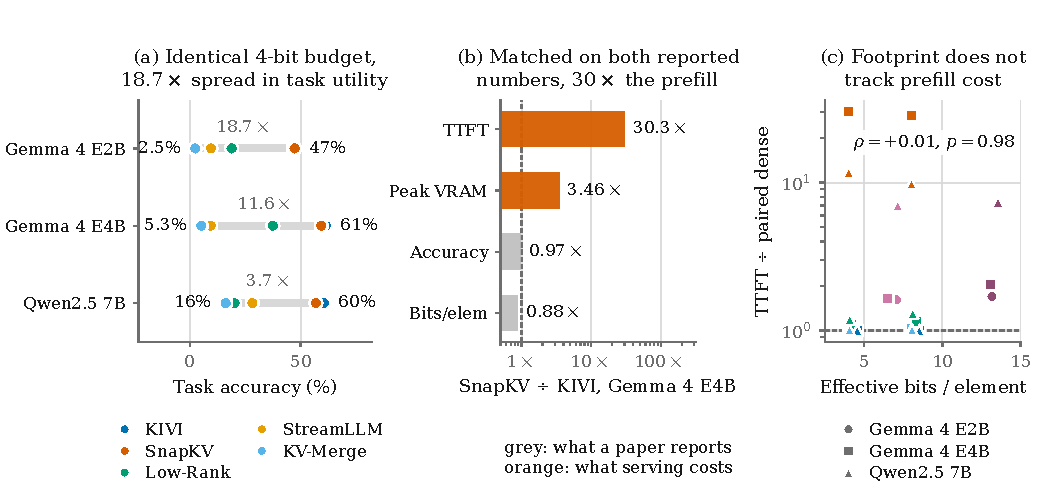
\includegraphics[width=\textwidth]{figures/fig1_decoupling.pdf}
\caption{\textbf{The two numbers a compression paper reports do not determine
what a serving system pays.}
\textbf{(a)} Five methods held at an identical nominal budget of 4 bits per KV
element --- realised payloads within $0.19$\bpt{} of one another, effective
footprints within $0.55$ once metadata is charged --- differ in task accuracy
by up to $18.7\times$. Selecting on bitrate alone leaves this entire range
undetermined.
\textbf{(b)} KIVI and SnapKV on Gemma~4 E4B agree on \emph{both} reported
numbers, to within $0.55$ bits per element and $2.0$ accuracy points, and then
diverge by $3.46\times$ in peak VRAM and $30.3\times$ in TTFT. Grey bars are
what a paper reports; orange bars are what the serving system pays.
\textbf{(c)} Over all 36 compressed operating points, effective footprint
carries no detectable signal about prefill cost. Marker shape denotes model,
colour denotes method.
Panel (b) reflects the SnapKV integration documented in
\S\ref{sec:provenance}, not SnapKV's fused reference kernel; the point is that
a serving system inherits the integration it can run, not the algorithm in the
abstract.}
\label{fig:decoupling}
\end{figure*}

\paragraph{Finding 1: at a fixed budget, the bitrate does not
order methods on task utility.}\label{M-find1}
Figure~\ref{fig:decoupling}(a) holds five methods at the same nominal 4-bit
budget: their realised payloads agree to within $0.19$ bits per element and
their effective footprints to within $0.55$, so any accuracy difference is
attributable to \emph{how} the budget is spent, not how much. Accuracy
nonetheless spans $2.5\%$ to $47.3\%$ on Gemma~4 E2B ($18.7\times$), $5.3\%$
to $61.3\%$ on Gemma~4 E4B ($11.6\times$) and $16.2\%$ to $60.4\%$ on
Qwen2.5~7B ($3.7\times$). Pooled over all 36 compressed configurations, the
rank correlation between memory saved and accuracy retained is
$\rho = {-}0.42$ ($p = 0.010$): saving more memory is, in these measurements,
if anything associated with retaining \emph{less} task ability.

\paragraph{Finding 2: matched on both reported numbers, serving
cost still differs by more than an order of magnitude.}\label{M-find2}
Figure~\ref{fig:decoupling}(b) takes two methods that agree on both reported
quantities --- within $0.55$ bits per element and $2.0$ accuracy points, on
the same model and the same prompts --- and finds them $3.46\times$ apart in
peak VRAM and $30.3\times$ apart in TTFT. This is a direct matched
observation, not a correlation over a scatter. Across configurations we detect
no rank relationship between memory saved and the measured hardware efficiency
multiplier ($\rho = {+}0.04$, $p = 0.84$) or between effective footprint and
prefill cost ($\rho = {+}0.01$, $p = 0.98$). We read these as the absence of a
\emph{detectable} relationship at this sample size, not as proof that none
exists; the matched comparison does not depend on them.

\paragraph{Finding 3: the reported footprint is itself
understated, unevenly.}\label{M-find3}
A representation's real cost is its payload \emph{plus} the metadata that
makes the payload decodable: quantisation scales and zero points, subspace
bases, eviction index tables, alignment padding. Charging for it moves a
factorised representation from a nominal $5.00$ to a realised $6.51$ bits per
element and a nominal 4-bit quantiser from $4.05$ to $4.55$ ---
understatements of $30\%$ and $12\%$, both flattering the method. Because the
overhead concentrates in particular families ($0.1\%$ for eviction,
$6$--$11\%$ for grouped quantisation, $10$--$23\%$ for factorised state)
rather than spreading evenly, correcting it does not merely rescale the
ranking, it reorders it.

\paragraph{Why this matters for serving systems.}\label{M-why}
Each finding breaks a decision a serving system actually makes.
\emph{Capacity planning} is sized from resident memory, and we observe peak
resident memory diverging from the analytic footprint by up to $3.46\times$ on
the same model, so a plan drawn from a compression ratio can err in the unsafe
direction. \emph{Latency objectives} are set on TTFT, and prefill-side
transformation work --- attention-score pooling, SVD, block factorisation ---
runs over the \emph{uncompressed} prompt before any saving materialises, which
no bitrate expresses. \emph{Mechanism selection} is per-deployment: the same
integration inflates TTFT $30.3\times$ on Gemma~4 E4B, $11.8\times$ on
Qwen2.5~7B and $1.04\times$ on Gemma~4 E2B, where its cost surfaces instead as
a $2.47\times$ peak-VRAM inflation --- so a single-model measurement would
have supported a confidently wrong generalisation in either direction. In
short, what a serving system runs is an \emph{implementation}, and its cost is
not recoverable from the algorithm's published ratio.

\paragraph{Contributions.}\label{M-contrib}
None of this is visible under existing practice, because task quality, memory
and latency are conventionally measured by different communities on different
workloads, so their disagreements never appear on the same row. Establishing
that they disagree requires measuring all three \emph{on the same query}, and
that measurement design --- not the summary scores it produces --- is what
makes the findings above credible.
\begin{itemize}[leftmargin=*,itemsep=2.0pt,topsep=3pt]
\item \textbf{An empirical characterisation of a three-way divergence that the
  field reports as two numbers} (\S\ref{sec:results}): at matched bitrate,
  accuracy varies up to $18.7\times$; at matched bitrate \emph{and} accuracy,
  serving cost varies $30.3\times$ in TTFT and $3.46\times$ in peak VRAM; over
  36 operating points we detect no rank association between representation
  footprint and realised hardware behaviour; and the divergence is itself
  model-dependent.
\item \textbf{\sys{}, the measurement methodology that makes that
  characterisation possible} (\S\ref{sec:sys}): a paired-execution primitive
  that runs every query twice, once under the 16-bit dense reference and once
  under the candidate, on the identical prompt in the same session, so that
  every ratio is formed against a baseline that cannot be differently
  configured or differently reported.
\item \textbf{An honest memory accounting} (\S\ref{sec:beff}): effective bits
  per element, charging each representation for the metadata without which its
  payload cannot be decoded, plus an explicit separation of
  \emph{analytically accounted} from \emph{physically realised} savings. This
  is load-bearing rather than pedantic: it shifts reported bitrates by
  $6$--$23\%$ and changes rankings.
\item \textbf{Per-method provenance and a reproducible pipeline}
  (\S\ref{sec:provenance}, Appendix~\ref{app:artifact}): for every method we
  state which code path produced its numbers and what that path does and does
  not represent, and we release the per-query records with scripts that
  regenerate every table, statistic and figure here.
\end{itemize}

\paragraph{What we do not claim.}\label{M-noclaim}
This is a controlled single-node study: three open-weight models (2B--7B), one
commodity GPU, batch size one, no continuous batching or paged attention. We
show that the reported-number-to-serving-cost mapping breaks in this regime
and quantify by how much; we do not claim the magnitudes transfer to other
model scales or to multi-tenant stacks, and \S\ref{sec:threats} is explicit
about the boundary. Concurrent work independently reports that compression
ratio is a poor predictor of end-to-end performance on a different model and
task set~\cite{agrawal2026benchmarking}; \S\ref{sec:related} states what our
measurement design adds to that observation.

% ===========================================================================
\section{Three Axes, and Why One Does Not Determine Another}
\label{sec:axes}

Current practice reports two numbers where a deployment decision needs three.
\emph{Representation efficiency} (Axis~1) is how many bits of state a method
keeps per KV element, \emph{including} everything needed to decode that state;
it is a property of the representation alone, it is what a compression ratio
tries to express, and it determines how much more context fits in a fixed
memory budget. \emph{Task utility} (Axis~2) is how much of the model's ability
survives the transform; it is a property of the representation \emph{and} the
model \emph{and} the task. \emph{Serving efficiency} (Axis~3) is what the
method costs in prefill latency, decode throughput and resident device memory
when actually executed; it is a property of the representation, its
\emph{implementation}, and the hardware. Only the first can be read off a
datasheet.

Axis~1 need not determine Axis~2 because two representations can keep the same
number of bits and spend them completely differently: a 4-bit quantiser spends
its budget uniformly over all tokens, an eviction policy spends 16 bits on a
quarter of the tokens and nothing on the rest, and a pooling scheme spends
them on averages that may correspond to no token the model needs. Which
allocation is right depends on where the task's information lies, which a bit
count cannot express.

Axis~1 need not determine Axis~3 for four reasons, each of which we measure.
\emph{(i) Metadata is neither free nor proportional.} Group-wise quantisation
stores a scale and zero point per group; a factorised scheme stores anchors
and bases; an eviction method needs only a position index. At a nominal 4-bit
budget these cost $11\%$, $23\%$ and $0.1\%$ of realised footprint
respectively (\S\ref{sec:res_metadata}), so a ratio computed on payload alone
mis-ranks them.
\emph{(ii) Prefill cost is decided by the transform, not the footprint.}
Attention-score pooling, SVD and block factorisation all do work proportional
to the \emph{uncompressed} prompt before any saving materialises; our measured
TTFT inflation spans $0.96\times$ to $30.3\times$ dense at effectively
identical footprints.
\emph{(iii) Implementation efficiency is part of the answer.} The same
algorithm as a fused kernel or as un-fused tensor operations is a different
serving proposition --- and it is the deployable artifact, not the algorithm,
that a serving system runs.
\emph{(iv) Peak memory is not resident memory.} A transform that ends smaller
can pass through a much larger intermediate; in our runs the method with the
smallest analytic footprint at 4 bits had the largest measured peak VRAM.

\noindent The three axes therefore have to be measured separately, on the same
queries. That is what \sys{} does.

% ===========================================================================
\section{\sys{}: Measuring the Three Axes on One Query}
\label{sec:sys}

\subsection{The paired execution primitive}

Let $\mathcal{M}$ be an autoregressive model with fixed weights,
$\mathcal{D} = \{(x_i, y_i, \tau_i, L_i)\}_{i=1}^N$ a set of queries with
targets, task types and context lengths, $\mathcal{R}_{\text{dense}}$ the
uncompressed 16-bit reference representation, and $\mathcal{A}(\mathcal{B})$ a
candidate representation under budget $\mathcal{B}$. The atomic unit of
measurement is the 4-tuple
$\mathcal{U}_i = (\mathcal{M},\,(x_i,y_i),\,\mathcal{R}_{\text{dense}},\,
\mathcal{A}(\mathcal{B}))$. For each unit \sys{} executes both
$\hat{y}_{i,\text{dense}} = \mathcal{M}(x_i \mid \mathcal{R}_{\text{dense}})$
and $\hat{y}_{i,\text{method}} = \mathcal{M}(x_i \mid \mathcal{A}(\mathcal{B}))$
on the identical prompt, and records for both the task score
$s \in [0,1]$, the analytic state footprint in bytes, and the measured TTFT,
decode throughput and peak device memory (Figure~\ref{fig:framework}).

Pairing at the query level rather than the dataset level is what makes the
three axes comparable. Every ratio we report --- accuracy, TTFT inflation,
VRAM inflation --- is formed against a dense execution of the same prompt in
the same session on the same device, so it cannot be contaminated by a
differently configured or differently reported baseline. It also means a
per-query anomaly is attributable: the dense and compressed outcomes for that
exact prompt are both on record.

\begin{figure*}[t]
\centering
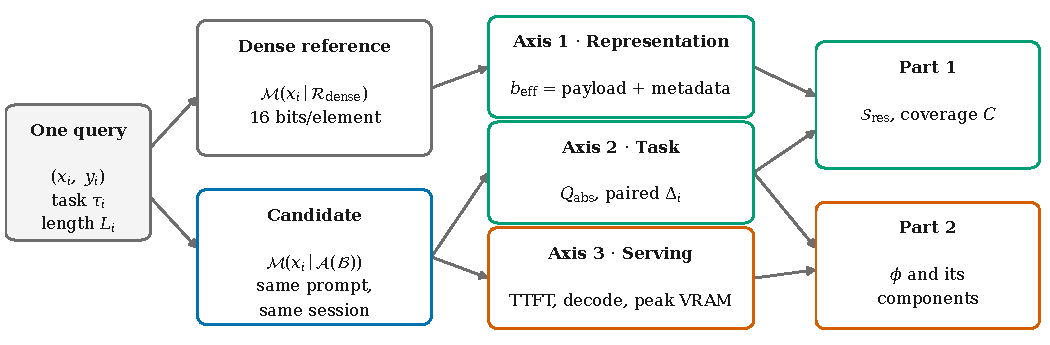
\includegraphics[width=\textwidth]{figures/fig2_framework.pdf}
\caption{\textbf{Every measurement in this paper is a difference between two
executions of the same prompt.} The dense reference is re-run for each query
rather than quoted from a previous session, which is what allows an accuracy
difference, a footprint difference and a latency difference to be attributed
to the representation rather than to the harness. Part~1 and Part~2 are
reported separately by design (\S\ref{sec:parts}).}
\label{fig:framework}
\end{figure*}

\subsection{Task quality}

For a completed candidate run with evaluator score
$s_{i,\text{method}} \in [0,1]$ we report absolute success,
$Q_{\text{abs},i} = 100\,s_{i,\text{method}}$ clipped to $[0,100]$, rather
than retention relative to dense. Retention rewards a method for being paired
with a weak baseline: a method scoring $20\%$ where dense scores $20\%$ has
$100\%$ retention and is useless. The paired dense outcome is still recorded
for every query --- it defines coverage, enables failure diagnosis, and lets a
reader recompute retention --- but it is not substituted into the headline
number. We log the signed paired difference
$\Delta_i = s_{i,\text{method}} - s_{i,\text{dense}}$ throughout.

\subsection{Memory accounting: effective bits per element}
\label{sec:beff}

This is the axis most often misreported, so we state the accounting
explicitly. The total state of a representation is
\begin{equation}
\label{eq:memory}
M_{\text{method}}(L) = \underbrace{M_{\text{algo}}(L)}_{\text{payload}}
                     + \underbrace{M_{\text{meta}}(L)}_{\text{scales, bases, indices}}
                     + \underbrace{M_{\text{align}}(L)}_{\text{padding}},
\end{equation}
and normalising the \emph{total} by the uncompressed element count gives
\begin{equation}
\label{eq:beff}
\beff = \frac{8 \cdot M_{\text{method}}(L)}
             {2 \, N_{\text{layers}} \, N_{\text{kv}} \, d_{\text{head}} \, L}
        \quad [\text{bits/element}],
\end{equation}
which is exactly $16.0$ for an uncompressed FP16/BF16 cache. Memory saving is
$R_{\text{mem}} = 100 \cdot \max(0,\, 1 - M_{\text{method}}/M_{\text{dense}})$.

A method's nominal bit-width describes only $M_{\text{algo}}$. The remaining
terms are not optional: without the scales the payload cannot be dequantised,
without the bases the projection cannot be inverted. They are also not uniform
across families --- group-wise quantisation pays per group, a subspace method
per block, an eviction method only a token index --- so omitting them does not
shift every method equally, it \emph{re-ranks} them
(\S\ref{sec:res_metadata}).

\paragraph{Analytic versus physically realised savings.}
We distinguish two things a compression result can mean. A saving is
\emph{physically realised} when the resident cache tensors actually shrink,
and \emph{analytically accounted} when the scheme's footprint is computed from
its definition while the harness retains the transformed values in a wider
dtype for exactness. Both are legitimate --- the first measures a system, the
second measures a representation --- but they are not interchangeable, and
conflating them is how a paper ends up claiming a serving win it did not
measure. \S\ref{sec:provenance} states which is which for every method here,
and every peak-VRAM number we report reflects what was physically resident.

\subsection{Two tracks, and which one carries the evidence}
\label{sec:parts}

\paragraph{Part 1 (representation and task).}
\begin{equation}
\label{eq:sres}
\Sres = \alpha \, Q_{\text{abs}} + (1 - \alpha)\, R_{\text{mem}},
\qquad \alpha = 0.70 \text{ by default}.
\end{equation}
The linear form is chosen for transparency, not optimality: it is monotone in
both arguments, bounded on $[0,100]$, Pareto consistent, and --- unlike a
product or harmonic form --- never lets one dimension annihilate the other, so
a reader can always decompose a score back into the two quantities that
produced it (Appendices~\ref{app:proofs} and~\ref{app:formulations}). At
$\alpha = 0.70$ one accuracy point is worth $2.33$ points of memory saving; we
report $\alpha$ sensitivity in Appendix~\ref{app:formulations} rather than
asking the reader to accept the default. Aggregation uses a byte-weighted
memory aggregate so that long contexts are not diluted by short ones, and
failed queries are charged the dense footprint and score zero rather than
being dropped (Appendix~\ref{app:protocol}). Paired coverage
$C = N_{\text{paired success}}/N_{\text{total}}$ is reported \emph{beside}
$\Sres$ rather than multiplied into it, so a run that failed for allocator
reasons stays distinguishable from one that completed and scored zero.
Coverage was $1.00$ for every configuration reported here.

\paragraph{Part 2 (measured serving).}
Part~2 records TTFT (wall-clock to first emitted token, including all
transform work), decode throughput $\mathcal{T}_{\text{dec}}$, and peak
resident device memory $\mathcal{P}$. Each is converted to a
paired efficiency against the \emph{same query's} dense execution,
\begin{equation}
\label{eq:phi_components}
\begin{aligned}
\phi_{\text{ttft}} &= \min\!\big(1,\ \text{TTFT}_{\text{dense}} / \text{TTFT}_{\text{method}}\big), \\[1pt]
\phi_{\text{thru}} &= \min\!\big(1,\ \mathcal{T}_{\text{method}} / \mathcal{T}_{\text{dense}}\big), \\[1pt]
\phi_{\text{vram}} &= \min\!\big(1,\ \mathcal{P}_{\text{dense}} / \mathcal{P}_{\text{method}}\big),
\end{aligned}
\end{equation}
and combined into a single \emph{hardware multiplier}
\begin{equation}
\label{eq:phi}
\phi = \phi_{\text{ttft}}^{0.35}\, \phi_{\text{thru}}^{0.35}\,
       \phi_{\text{vram}}^{0.30} \in (0, 1].
\end{equation}
The weights give interactive responsiveness slightly more emphasis than
resident footprint; we make no claim this is the only defensible weighting,
and the components are always reported separately so a reader can reweight.
$\phi$ is computed per query and then averaged.

\paragraph{$\phi$ is the serving axis; $\Ssys$ is only a convenience.}
\textbf{$\phi$ contains no term from Part~1.} It is built entirely from
paired latency, throughput and memory measurements, and it is therefore the
quantity to use whenever the question is whether algorithmic utility predicts
serving behaviour. For readers who want a single ordering we also report
\begin{equation}
\label{eq:ssys}
\Ssys = \alpha \Sres + (1-\alpha) \cdot 100\phi ,
\end{equation}
but $\Ssys$ is a presentational summary, \emph{not} evidence: it is defined in
terms of $\Sres$, so any correlation between the two is circular by
construction and we never compute one. Every independence claim in this paper
is made against $\phi$. One consequence is worth flagging in advance: the
rank displacements we report in \S\ref{sec:res_serving} between the $\Sres$
ordering and the $\Ssys$ ordering are a \emph{lower bound} on the disagreement
between the axes, precisely because the two orderings share the $\Sres$ term.
Nothing in the paper's argument would change if $\Ssys$ were deleted; it is
retained only because a single column is convenient to scan.

% ===========================================================================
\section{Study Design}
\label{sec:setup}

\paragraph{Design.}
Each model is evaluated on $5$ tasks $\times$ $5$ context lengths $\times$ $3$
samples $= 75$ distinct queries. Each query is executed under $14$
configurations: five fixed-budget methods at nominal budgets of $4$ and $8$
bits per element, two adaptive factorised configurations, and the dense
reference (recorded in both budget sweeps). That is $1{,}050$ paired
executions per model and $3{,}150$ in total. Decoding is greedy ($T=0$) and
the generation budget is fixed per task ($32$--$256$ new tokens) and identical
across every configuration, so no method is advantaged by a longer or shorter
budget. We report operating points separately rather than pooling the two
budget sweeps into one row per method: a pooled ``$\approx$\,6 bits'' row
averages two configurations whose accuracies can differ by more than $30$
points, and it is precisely the matched-budget comparison that carries the
evidence.

\paragraph{Models and context ladders.}
Gemma~4 E2B (\texttt{google/\allowbreak gemma-4-e2b-it}) at $2$K, $8$K,
$32$K, $64$K, $128$K; Gemma~4 E4B (\texttt{google/\allowbreak gemma-4-e4b-it})
and Qwen2.5~7B (\texttt{Qwen/\allowbreak Qwen2.5-7B-Instruct}) at $2$K, $4$K,
$8$K, $16$K, $32$K.

\paragraph{Tasks.}
Single-needle and multi-needle retrieval at parameterised
depths~\cite{kamradt2023needle}; RULER key--value lookup among distractors and
RULER multi-step variable tracking~\cite{hsieh2024ruler}; and synthetic
cross-document multi-hop QA. Two of the five behave as controls rather than
discriminators in our study, and \S\ref{sec:res_tasks} treats them as such.

\paragraph{Environment.}
A single NVIDIA GeForce RTX 4070 SUPER ($12$\,GB VRAM), PyTorch $2.6.0$
(CUDA 12.4 build), \texttt{transformers} $5.15.1$, Python $3.12.10$, Windows
11. Weights were loaded in 4-bit NormalFloat via bitsandbytes so that the
weight footprint is held constant and the $128$K ladder fits in $12$\,GB; the
KV cache under study is unaffected by that choice. Prefill used chunked
forward passes ($4{,}096$ tokens) to avoid intermediate allocation spikes.
Absolute latencies are hardware-specific, but because every comparison is
paired against a dense execution on the same device in the same session, the
reported ratios are not distorted by machine-to-machine variation.

\paragraph{Determinism.}
The dense reference was executed twice for every query, once in each budget
sweep, which gives a free replication check: on Gemma~4 E4B and Qwen2.5~7B all
$150$ re-executions produced byte-identical outputs, and on Gemma~4 E2B
exactly one query of $75$ changed score. Run-to-run variance is negligible at
the resolution of our claims (Appendix~\ref{app:protocol}).

\subsection{Methods and provenance}
\label{sec:provenance}

Table~\ref{tab:provenance} states, for every method, which implementation
produced its numbers and whether its memory saving was physically realised or
analytically accounted. We treat this disclosure as part of the result rather
than an appendix detail: a serving claim is only as strong as the code path
that produced it.

\begin{table*}[t]
\centering
\small
\setlength{\tabcolsep}{4.0pt}
\caption{\textbf{A serving number is a property of a code path, so we say
which one.} ``Upstream'' means the authors' released code was invoked;
``harness'' means a reference implementation written for this study following
the published scheme. ``Realised'' means the resident cache tensors physically
shrank; ``analytic'' means the footprint was computed from the scheme while
values were retained in a wider dtype, so quality is exact for the scheme but
no device memory was freed.}
\label{tab:provenance}
\begin{tabular}{@{}llll p{9.4cm}@{}}
\toprule
\textbf{Method} & \textbf{Impl.} & \textbf{Saving} & \textbf{Budget} & \textbf{What the measured numbers do and do not represent} \\
\midrule
KIVI (INT4/INT8) & harness & analytic & 4, 8 &
Asymmetric grouped min--max, per-channel keys, per-token
values~\cite{liu2024kivi}; partial key groups stay at 16 bits and are charged
as such. Quality is exact for the scheme; its favourable $\phi$ reflects a
cheap transform, not a production integer kernel. \\[2pt]
SnapKV & upstream & realised & 4, 8 &
\texttt{SnapKVCluster.update\_kv} at \texttt{e216ddc}. Upstream's monkeypatch
targets \texttt{transformers}~4.37 and Llama/Mistral only, so under
\texttt{transformers}~5.x the cluster is driven directly, \emph{outside} the
fused attention path. Its TTFT is a property of that integration, not of
SnapKV's achievable latency. \\[2pt]
StreamingLLM & upstream & realised & 4, 8 &
\texttt{StartRecentKVCache} at \texttt{2e50426}; policy unmodified. \\[2pt]
KV-Merging & harness & realised & 4, 8 &
Temporal mean-pooling of consecutive states, sinks and recent window
preserved~\cite{ge2023model}. \\[2pt]
Low-Rank KV & harness & analytic & 4, 8 &
Per-head mean-centred truncated SVD~\cite{sharma2023truth}; footprint is the
$U,\Sigma,V$ factor size. \\[2pt]
DKV-Mid / DKV-High & upstream & analytic & adaptive &
Anchor-plus-low-rank differential compression~\cite{dkvpreprint}. The
block compressor is driven over the resident cache; the repository's paged
serving runtime and decode kernel were unavailable on this platform, so these
numbers characterise the \emph{representation}, not that runtime's decode
speedup. \\[2pt]
Dense FP16 & --- & --- & 16 & Uncompressed paired reference. \\
\bottomrule
\end{tabular}
\end{table*}

Two caveats deserve to be read before any serving number in this paper.
Driven outside its fused attention path, SnapKV's observation-window pooling
runs as separate tensor operations over the full prompt, which is why its
measured prefill cost is large. We report it because it is the honest
measurement of the code path that was runnable here, and because it is a
direct instance of the paper's own thesis: serving efficiency is a property of
an algorithm \emph{and} its implementation, and is therefore not predictable
from a compression ratio. It must not be read as a claim about SnapKV's
achievable latency. The same caveat applies in the opposite direction to DKV:
its representation is measured, its serving runtime is not.

% ===========================================================================
\section{Results}
\label{sec:results}

The three subsections below take the three questions of \S\ref{sec:intro} in
turn. Table~\ref{tab:threeaxis} is the study in one grid --- all three axes at
every operating point, for all three models --- and every comparison drawn
below can be read off it directly.

\begin{table*}[t]
\centering
\small
\setlength{\tabcolsep}{4.2pt}
\caption{\textbf{Reading across a row shows the three axes disagreeing.}
$b_{\text{pay}}$ is the compressed payload alone --- the quantity
conventionally reported --- and $\beff$ additionally charges mandatory
metadata (Eq.~\ref{eq:beff}); ``meta'' is the metadata share of realised
footprint. ``$\times$dense'' is the mean per-query TTFT ratio against that
query's own dense execution. $\phi$ (Eq.~\ref{eq:phi}) is the pure hardware
term and carries the serving evidence; $\Ssys$ is the convenience summary of
\S\ref{sec:parts} and is not used as evidence anywhere. Best $\Sres$ and best
$\phi$ per model in \textbf{bold} ($\phi$ excluding the dense reference, which
is $1.00$ by definition). Serving figures reflect the implementations in
Table~\ref{tab:provenance}. Paired coverage was $1.00$ throughout.}
\label{tab:threeaxis}
\begin{tabular}{@{}ll rrr rr rrrr rr@{}}
\toprule
& & \multicolumn{3}{c}{\textbf{Axis 1: representation}} & \multicolumn{2}{c}{\textbf{Axis 2: task}} & \multicolumn{4}{c}{\textbf{Axis 3: measured serving}} & \\
\cmidrule(lr){3-5}\cmidrule(lr){6-7}\cmidrule(lr){8-11}
\textbf{Method} & \textbf{Bits} & $b_{\text{pay}}$ & $\beff$ & meta & Acc. & $\Sres$ & TTFT & $\times$dense & Dec. & VRAM & $\phi$ & $\Ssys$ \\
 & & & & (\%) & (\%) & & (s) & & (tok/s) & (MB) & & \\
\midrule
\multicolumn{13}{@{}l}{\textit{Gemma 4 E2B} \ (2K--128K)} \\[1pt]
KIVI & 4 & 4.01 & 4.51 & 11.1 & 46.7 & 54.2 & 12.51 & 1.00$\times$ & 12.1 & 846 & \textbf{0.97} & 67.1 \\
KIVI & 8 & 8.01 & 8.51 & 5.9 & 46.2 & 46.4 & 12.51 & 1.00$\times$ & 11.7 & 848 & 0.96 & 61.2 \\
SnapKV & 4 & 4.00 & 4.01 & 0.2 & 47.3 & \textbf{55.6} & 13.02 & 1.04$\times$ & 12.8 & 2088 & 0.71 & 60.2 \\
SnapKV & 8 & 8.00 & 8.02 & 0.2 & 46.2 & 47.3 & 13.06 & 1.04$\times$ & 13.0 & 2088 & 0.71 & 54.4 \\
Low-Rank & 4 & 4.05 & 4.05 & 0.0 & 18.9 & 35.7 & 12.76 & 1.02$\times$ & 12.3 & 849 & 0.92 & 52.5 \\
Low-Rank & 8 & 8.09 & 8.09 & 0.0 & 43.6 & 45.3 & 12.84 & 1.02$\times$ & 12.2 & 851 & 0.91 & 59.1 \\
StreamLLM & 4 & 4.00 & 4.01 & 0.2 & 9.6 & 29.2 & 12.58 & 1.00$\times$ & 13.6 & 847 & 0.95 & 48.8 \\
StreamLLM & 8 & 8.00 & 8.02 & 0.2 & 36.1 & 40.2 & 12.58 & 1.00$\times$ & 13.7 & 848 & 0.95 & 56.7 \\
KV-Merge & 4 & 4.01 & 4.02 & 0.4 & 2.5 & 24.2 & 12.60 & 1.00$\times$ & 14.0 & 848 & 0.95 & 45.3 \\
KV-Merge & 8 & 8.01 & 8.04 & 0.4 & 24.0 & 31.7 & 12.57 & 1.00$\times$ & 13.5 & 848 & 0.95 & 50.6 \\
DKV-Mid & adapt. & 5.46 & 7.07 & 22.8 & 44.7 & 48.0 & 22.26 & 1.61$\times$ & 13.8 & 1390 & 0.84 & 58.9 \\
DKV-High & adapt. & 10.78 & 13.17 & 18.1 & 46.7 & 38.0 & 23.40 & 1.70$\times$ & 13.8 & 1391 & 0.83 & 51.4 \\
Dense FP16 & -- & 16.00 & 16.00 & 0.0 & 46.4 & 32.5 & 13.18 & 1.00$\times$ & 13.4 & 1118 & 1.00 & 52.8 \\
\midrule
\multicolumn{13}{@{}l}{\textit{Gemma 4 E4B} \ (2K--32K)} \\[1pt]
KIVI & 4 & 4.05 & 4.55 & 10.9 & 61.3 & \textbf{64.4} & 2.84 & 1.00$\times$ & 12.8 & 761 & \textbf{0.99} & 74.7 \\
KIVI & 8 & 8.03 & 8.53 & 5.8 & 62.7 & 57.9 & 2.84 & 1.00$\times$ & 12.8 & 761 & 0.99 & 70.1 \\
SnapKV & 4 & 4.00 & 4.00 & 0.1 & 59.3 & 64.0 & 86.04 & 30.26$\times$ & 11.2 & 2632 & 0.48 & 59.1 \\
SnapKV & 8 & 8.00 & 8.01 & 0.1 & 60.7 & 57.5 & 80.73 & 28.39$\times$ & 10.0 & 2632 & 0.47 & 54.4 \\
Low-Rank & 4 & 4.19 & 4.19 & 0.0 & 37.5 & 48.4 & 3.11 & 1.09$\times$ & 13.1 & 761 & 0.93 & 61.9 \\
Low-Rank & 8 & 8.34 & 8.34 & 0.0 & 60.0 & 56.4 & 3.25 & 1.14$\times$ & 13.0 & 761 & 0.91 & 66.7 \\
StreamLLM & 4 & 4.00 & 4.00 & 0.1 & 9.5 & 29.1 & 2.92 & 1.03$\times$ & 13.6 & 761 & 0.97 & 49.4 \\
StreamLLM & 8 & 8.00 & 8.01 & 0.1 & 41.4 & 44.0 & 2.91 & 1.02$\times$ & 13.6 & 762 & 0.97 & 59.8 \\
KV-Merge & 4 & 4.03 & 4.04 & 0.2 & 5.3 & 26.1 & 2.91 & 1.02$\times$ & 13.7 & 761 & 0.97 & 47.3 \\
KV-Merge & 8 & 8.02 & 8.04 & 0.2 & 45.3 & 46.7 & 2.92 & 1.03$\times$ & 13.3 & 762 & 0.97 & 61.6 \\
DKV-Mid & adapt. & 5.00 & 6.51 & 23.2 & 55.3 & 56.5 & 5.06 & 1.65$\times$ & 12.3 & 761 & 0.84 & 64.8 \\
DKV-High & adapt. & 10.68 & 13.07 & 18.3 & 61.3 & 48.4 & 6.25 & 2.03$\times$ & 12.2 & 761 & 0.85 & 59.3 \\
Dense FP16 & -- & 16.00 & 16.00 & 0.0 & 64.0 & 44.8 & 2.96 & 1.00$\times$ & 12.4 & 761 & 1.00 & 61.4 \\
\midrule
\multicolumn{13}{@{}l}{\textit{Qwen2.5 7B} \ (2K--32K)} \\[1pt]
KIVI & 4 & 4.05 & 4.55 & 10.9 & 60.4 & \textbf{63.8} & 5.47 & 1.00$\times$ & 16.4 & 3854 & 0.98 & 74.1 \\
KIVI & 8 & 8.04 & 8.53 & 5.8 & 60.9 & 56.6 & 5.46 & 1.00$\times$ & 16.4 & 3854 & 0.98 & 69.2 \\
SnapKV & 4 & 4.00 & 4.01 & 0.2 & 56.9 & 62.3 & 64.08 & 11.77$\times$ & 24.3 & 5128 & 0.79 & 67.4 \\
SnapKV & 8 & 8.00 & 8.02 & 0.2 & 59.6 & 56.7 & 53.30 & 9.79$\times$ & 20.0 & 5137 & 0.77 & 62.6 \\
Low-Rank & 4 & 4.07 & 4.07 & 0.0 & 20.2 & 36.5 & 6.49 & 1.19$\times$ & 18.2 & 3854 & 0.91 & 52.8 \\
Low-Rank & 8 & 8.10 & 8.10 & 0.0 & 36.9 & 40.6 & 7.14 & 1.31$\times$ & 18.0 & 3854 & 0.87 & 54.4 \\
StreamLLM & 4 & 4.00 & 4.01 & 0.2 & 28.3 & 42.3 & 5.50 & 1.01$\times$ & 27.1 & 3854 & 0.99 & 59.3 \\
StreamLLM & 8 & 8.00 & 8.02 & 0.2 & 44.8 & 46.3 & 5.53 & 1.02$\times$ & 22.8 & 3854 & 0.99 & 62.1 \\
KV-Merge & 4 & 4.03 & 4.05 & 0.4 & 16.2 & 33.8 & 5.51 & 1.01$\times$ & 28.1 & 3854 & \textbf{0.99} & 53.4 \\
KV-Merge & 8 & 8.02 & 8.05 & 0.4 & 23.5 & 31.4 & 5.52 & 1.01$\times$ & 23.6 & 3854 & 0.99 & 51.7 \\
DKV-Mid & adapt. & 5.84 & 7.15 & 18.3 & 53.3 & 53.9 & 39.55 & 6.97$\times$ & 15.3 & 3854 & 0.70 & 58.8 \\
DKV-High & adapt. & 12.14 & 13.55 & 10.4 & 59.1 & 46.0 & 41.88 & 7.38$\times$ & 15.3 & 3854 & 0.73 & 54.0 \\
Dense FP16 & -- & 16.00 & 16.00 & 0.0 & 60.0 & 42.0 & 5.56 & 1.00$\times$ & 16.3 & 3854 & 1.00 & 59.4 \\
\bottomrule
\end{tabular}

\end{table*}

\subsection{Does the bitrate order methods on task utility?}
\label{sec:res_task}

Holding the nominal budget fixed isolates Axis~1 from Axis~2: at $4$ bits the
five fixed-budget methods realise payloads within $0.19$ bits per element of
one another, and effective footprints within $0.55$ once metadata is charged,
so any accuracy difference between them is attributable to how the budget is
spent rather than how much.

The differences are large. On Gemma~4 E2B accuracy at $4$ bits ranges from
$2.5\%$ (KV-Merging) to $47.3\%$ (SnapKV), a factor of $18.7$; on Gemma~4 E4B
from $5.3\%$ to $61.3\%$ ($11.6\times$); on Qwen2.5~7B from $16.2\%$ to
$60.4\%$ ($3.7\times$). At $8$ bits the spreads narrow but remain substantial
($22.2$, $21.2$ and $37.4$ accuracy points respectively), because the methods
that fail at $4$ bits recover unevenly: StreamingLLM gains $26.5$ points on
E2B between the two budgets while KIVI gains none ($46.7\% \to 46.2\%$, within
noise). How much accuracy a bit buys is itself method-dependent.

Table~\ref{tab:matched} shows the same comparison across models, and the
ordering is not stable: Low-Rank KV is third at 4 bits on the two Gemma models
and fourth on Qwen2.5~7B, where StreamingLLM passes it; and at 8 bits
StreamingLLM is last of the five on Gemma~4 E4B ($41.4\%$) yet third on
Qwen2.5~7B ($44.8\%$). Pooled over all $36$ compressed
operating points the rank correlation between memory saved and accuracy is
$\rho = {-}0.42$ ($p = 0.010$); per model it is ${-}0.28$, ${-}0.64$ and
${-}0.39$. The negative sign is unsurprising --- within a family, saving more
costs accuracy --- but what matters here is the absence of any positive
predictive relationship \emph{across} families. In these measurements, a
bitrate is not sufficient to order these methods on task ability, even
approximately.

\begin{table}[t]
\centering
\small
\setlength{\tabcolsep}{4.0pt}
\caption{\textbf{Identical budget, three models, and no stable ordering.}
Accuracy per model at each controlled nominal budget, with the mean realised
$\beff$, mean paired TTFT inflation and mean hardware multiplier over the
three models. Within a block every method holds the same nominal budget, so
accuracy differences are attributable to how the budget is spent, and the
serving columns to how the transform is implemented.}
\label{tab:matched}
\begin{tabular}{@{}l ccc c cc@{}}
\toprule
& \multicolumn{3}{c}{\textbf{Task accuracy (\%)}} & & \multicolumn{2}{c}{\textbf{Serving}} \\
\cmidrule(lr){2-4}\cmidrule(lr){6-7}
\textbf{Method} & E2B & E4B & 7B & $\beff$ & TTFT & $\phi$ \\
\midrule
\multicolumn{7}{@{}l}{\textit{Identical nominal budget: 4~bits/element}} \\[1pt]
KIVI & 46.7 & 61.3 & 60.4 & 4.54 & 1.00$\times$ & 0.98 \\
SnapKV & 47.3 & 59.3 & 56.9 & 4.01 & 14.36$\times$ & 0.66 \\
Low-Rank & 18.9 & 37.5 & 20.2 & 4.11 & 1.10$\times$ & 0.92 \\
StreamLLM & 9.6 & 9.5 & 28.3 & 4.01 & 1.01$\times$ & 0.97 \\
KV-Merge & 2.5 & 5.3 & 16.2 & 4.04 & 1.01$\times$ & 0.97 \\
\midrule
\multicolumn{7}{@{}l}{\textit{Identical nominal budget: 8~bits/element}} \\[1pt]
KIVI & 46.2 & 62.7 & 60.9 & 8.52 & 1.00$\times$ & 0.98 \\
SnapKV & 46.2 & 60.7 & 59.6 & 8.01 & 13.08$\times$ & 0.65 \\
Low-Rank & 43.6 & 60.0 & 36.9 & 8.18 & 1.16$\times$ & 0.90 \\
StreamLLM & 36.1 & 41.4 & 44.8 & 8.01 & 1.01$\times$ & 0.97 \\
KV-Merge & 24.0 & 45.3 & 23.5 & 8.04 & 1.01$\times$ & 0.97 \\
\bottomrule
\end{tabular}

\end{table}

\subsection{How much does the metadata cost?}
\label{sec:res_metadata}

Figure~\ref{fig:effbits} decomposes every operating point into payload and
mandatory metadata. The overhead is strongly method-dependent. Eviction and
pooling methods store only a token index and pay $0.1$--$0.4\%$. Grouped
quantisation pays for scales and zero points: a nominal $4$-bit configuration
realises $4.51$--$4.55$ bits per element ($11\%$ overhead), and because the
metadata is per group rather than per bit, the same scheme at $8$ bits pays
only $5.8$--$5.9\%$. The factorised representations pay most --- $18$--$23\%$
on the two Gemma models and $10$--$18\%$ on Qwen2.5~7B ---
moving DKV-Mid from a nominal $5.00$ to a realised $6.51$ bits per element on
Gemma~4 E4B and DKV-High from $10.68$ to $13.07$ --- at which point it saves
$18\%$ of the dense footprint rather than the $33\%$ a payload-only accounting
would report.

This matters for ranking, not only for absolute numbers. Because the overhead
concentrates in one family, charging for it reorders the table: on Gemma~4
E4B, DKV-Mid falls from third to fifth of thirteen operating points, passed by
both 8-bit configurations it had outranked; on Gemma~4 E2B and Qwen2.5~7B,
DKV-High falls one position, passed by 8-bit StreamingLLM. The eviction and
pooling methods are barely charged at all, having almost nothing to charge, so
where one of them moves it is because a quantised or factorised neighbour fell
past it rather than because its own footprint changed. We note that the
correction is largest for the family whose numbers it most penalises, and we
report it in that direction because that is what the accounting yields.

\begin{figure*}[t]
\centering
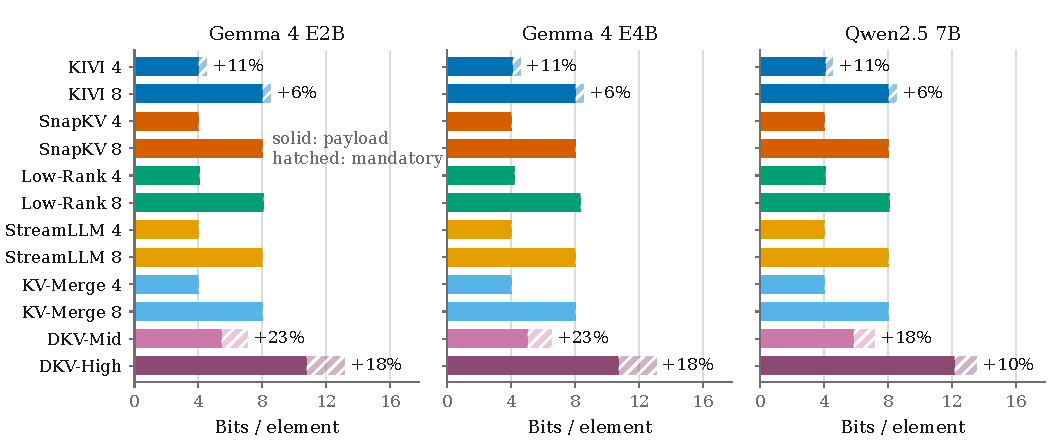
\includegraphics[width=\textwidth]{figures/fig3_effective_bits.pdf}
\caption{\textbf{The bits a method is charged for and the bits it actually
needs are not the same number, and the gap is family-specific.} Solid bars are
the compressed payload conventionally reported as the compression ratio;
hatched caps are the metadata without which the payload cannot be decoded.
Labels give the metadata share where it exceeds $5\%$. Because eviction
carries almost none and factorised state carries $10$--$23\%$, a payload-only
ratio does not merely understate footprint --- it reorders methods against one
another.}
\label{fig:effbits}
\end{figure*}

\subsection{Does task utility predict serving efficiency?}
\label{sec:res_serving}

The clearest evidence is a matched pair rather than a correlation. On Gemma~4
E4B at a $4$-bit budget, KIVI and SnapKV agree closely on both conventionally
reported numbers --- $4.55$ versus $4.00$ bits per element, $61.3\%$ versus
$59.3\%$ accuracy --- and then diverge completely on the third axis: TTFT of
$2.84$\,s versus $86.04$\,s ($30.3\times$), peak VRAM of $761$\,MB versus
$2{,}632$\,MB ($3.46\times$), and hardware multiplier $\phi$ of $0.99$ versus
$0.48$. The same pair on Qwen2.5~7B differs by $11.7\times$ in TTFT. Nothing
in Axis~1 or Axis~2 anticipates a $30\times$ prefill gap.

Across all operating points the association is not merely weak; it is not
detectable at all at this sample size.
Memory saved has no rank relationship to the measured hardware multiplier
($\rho = {+}0.04$, $p = 0.84$); effective footprint has none to TTFT inflation
($\rho = {+}0.01$, $p = 0.98$) or to measured peak-VRAM inflation
($\rho = {-}0.08$, $p = 0.63$). Within each model, algorithmic utility is if
anything mildly \emph{anti}-correlated with hardware efficiency
($\rho(\Sres, \phi) = {-}0.33$, ${-}0.30$, ${-}0.49$), which is what one would
expect if the methods that work hardest to preserve quality also do the most
work at prefill. With $12$--$13$ points per model these are descriptive
summaries of a small sample; we quote them to indicate the absence of a
detectable relationship, not to assert that none exists.

Consequently the two tracks order methods differently. Moving from the $\Sres$
ordering to the $\Ssys$ ordering shifts a configuration by $1.4$, $2.6$ and
$1.4$ positions on average for the three models; the largest single move is
SnapKV at $4$ bits on Gemma~4 E4B, second of thirteen on representation
utility and tenth on the serving summary. As noted in \S\ref{sec:parts}, these
displacements understate the disagreement, because $\Ssys$ embeds $\Sres$.

\paragraph{Where the multiplier is lost, and why it is model-dependent.}
Figure~\ref{fig:hardware}(b) separates the two ways $\phi$ falls: losses are
either prefill-bound (SnapKV on Gemma~4 E4B and Qwen2.5~7B, DKV on
Qwen2.5~7B) or peak-memory-bound (SnapKV on Gemma~4 E2B), and in no case are
they predictable from a method's position in Figure~\ref{fig:effbits}.
Figure~\ref{fig:hardware}(a) makes the model dependence explicit: the same
integration inflates TTFT by $30.3\times$, $11.8\times$ and $1.04\times$ on
the three models, and on the third its cost surfaces instead as a
$2.47\times$ peak-VRAM inflation ($\phi = 0.71$). Because the transform's cost
rides on the model's prompt-processing profile, the same code path lands
differently on different architectures. Methodologically this is the sharpest
of our results: a single-model systems measurement of a compression mechanism
does not transfer, and reporting one would have supported a confidently wrong
generalisation in either direction.

\begin{figure*}[t]
\centering
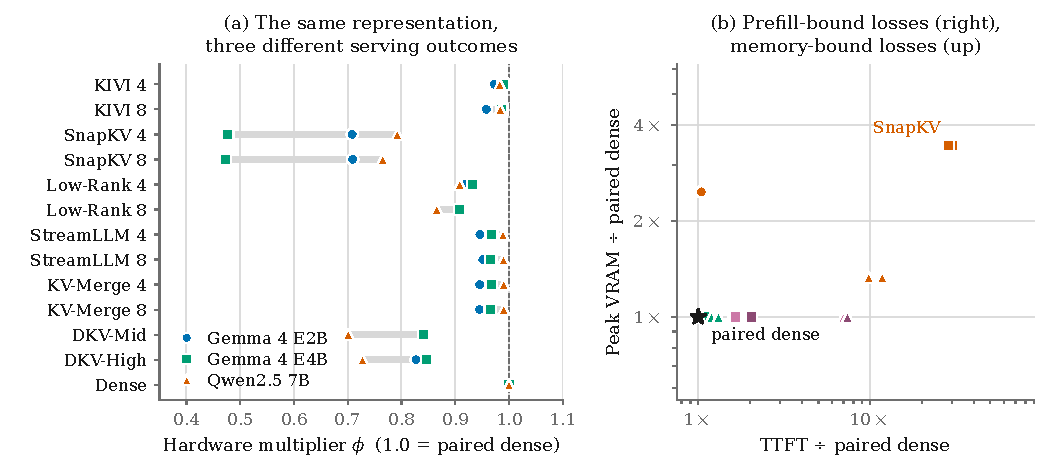
\includegraphics[width=\textwidth]{figures/fig4_hardware.pdf}
\caption{\textbf{The serving cost of a representation is a property of the
deployment, not of the representation.} \textbf{(a)} $\phi$ for every
operating point, one marker per model; a long grey bar is a method whose
serving behaviour changed substantially when only the model changed.
\textbf{(b)} The same points resolved into the two ways $\phi$ is lost: to the
right are prefill-bound losses, upward are peak-memory-bound losses. SnapKV
loses on different axes on different models. Neither panel is predictable from
Figure~\ref{fig:effbits}.}
\label{fig:hardware}
\end{figure*}

\subsection{Where the limit is the model, not the representation}
\label{sec:res_tasks}

Two features of the suite bound what its accuracy axis can resolve, and both
are visible only because a dense run was paired with every query. First, every
method scores $0.0\%$ on RULER multi-step variable tracking on all three
models --- \emph{including the uncompressed dense reference} (a single KIVI
configuration on Qwen2.5~7B reaches $3.3\%$). Whatever fails there is not the
representation, and without the paired dense run it would read as a
compression failure. Because the task is one of five it depresses every
reported average by roughly a fifth uniformly, changing no ranking. Second,
dense accuracy on multi-needle retrieval is $32$--$33\%$ on all three models,
consistent with partial credit for locating a subset of the planted needles,
so that task has little headroom to discriminate. Effectively three of five
tasks carry the discriminative signal, and absolute accuracies here should be
read with that in mind (Appendix~\ref{app:detail},
Figure~\ref{fig:heatmap}).

The same argument applies along context length. Over the full $2$K--$128$K
ladder on Gemma~4 E2B (Figure~\ref{fig:context}), dense accuracy is flat to
$32$K, falls at $64$K and drops sharply at $128$K, while the better compressed
methods track it throughout without the gap widening systematically. The
degradation beyond $64$K is therefore shared with the uncompressed baseline
and belongs to the model's usable context, not to compression --- a
distinction visible only because the dense reference was re-run at every
context length rather than assumed flat.

% ===========================================================================
\section{Implications for Serving Systems}
\label{sec:discussion}

\paragraph{Three numbers, not two.}
The minimum honest summary of a KV-compression mechanism is its effective bits
per element \emph{including} metadata, its task accuracy against a paired
dense run of the same model, and its measured TTFT, throughput and peak memory
relative to that same run. Each of the three carries information the other two
do not: reporting a nominal bit-width understates real footprint by
$6$--$23\%$ in a family-dependent way; reporting a ratio without task
measurement leaves an $18.7\times$ accuracy range undetermined; reporting both
without a systems measurement leaves a $30\times$ prefill range undetermined.

\paragraph{Which axis binds depends on the deployment.}
If the binding constraint is context length within a fixed memory budget,
Axis~1 with honest metadata accounting is the right selector. If it is answer
quality, Axis~2 must be measured on the target model, because the ordering of
methods changed across our three. If it is interactive latency or serving
cost, only Axis~3 is decisive, and it must be measured on the implementation
that will actually be deployed --- our SnapKV and DKV measurements illustrate,
in both directions, how far an integration can sit from an algorithm's
potential.

\paragraph{Prefill cost deserves first-class accounting.}
A compression mechanism that shrinks the cache but adds a pass over the
uncompressed prompt trades decode-side memory for prefill-side latency. In a
disaggregated serving stack~\cite{zhong2024distserve} that trade lands on a
different machine from the one it benefits, and under chunked
prefill~\cite{agrawal2024sarathi} it competes directly with the decode batch
for the same scheduling budget. Neither effect is expressible in a compression
ratio. We report TTFT with device synchronisation around the full
prefill-plus-transform-plus-first-token path, so that transform cost is
charged to the method that incurs it, and we recommend the same convention.

\paragraph{Keep the tracks apart.}
We report $\Sres$ and $\phi$ separately and decline to average them, because
their disagreement is the finding: a single score would have concealed that a
configuration ranked second on representation utility ranks tenth on serving.

% ===========================================================================
\section{Threats to Validity and Scope}
\label{sec:threats}

We state these as constraints on what our evidence supports, not as future
work.

\begin{enumerate}[leftmargin=*,itemsep=2.0pt,topsep=3pt]
\item \textbf{Implementation, not algorithm.} Axis~3 measures code paths.
  Where an upstream fused kernel was unavailable on our platform --- SnapKV's
  patched attention, DKV's paged runtime --- our numbers characterise the
  integration that ran and are not upper bounds on those algorithms
  (Table~\ref{tab:provenance}). This is intrinsic to serving measurement
  rather than incidental to our setup: there is no implementation-independent
  serving number.
\item \textbf{Analytic versus realised savings.} For KIVI and Low-Rank KV the
  footprint is analytically accounted while values are retained in a wider
  dtype, so their Part~1 savings are exact for the scheme but no device memory
  was freed, and their favourable $\phi$ reflects a cheap transform rather
  than a production integer kernel. For SnapKV, StreamingLLM and KV-Merging
  the cache physically shrinks and both tracks are measured end to end.
\item \textbf{Three models, two families, 2B--7B.} Method orderings already
  differ across Gemma~4 E2B/E4B and Qwen2.5~7B, which is itself a reason not
  to extrapolate to 13B+ or 70B+ models, to different attention layouts, or to
  other tokenisers.
\item \textbf{Single-GPU, single-stream.} One RTX 4070 SUPER, batch size one,
  no tensor or pipeline parallelism, no continuous batching, no paged
  attention. Multi-tenant serving changes the memory--latency trade-off
  substantially and our Axis~3 magnitudes do not transfer to it unexamined;
  what we do claim is that a divergence this large at batch size one cannot be
  assumed to disappear in a multi-tenant stack.
\item \textbf{Retrieval-weighted synthetic tasks.} The suite probes retrieval,
  associative lookup and short multi-hop reasoning, not summarisation,
  open-ended generation, agentic dialogue or code, where the information a
  compressed cache must preserve is distributed differently. Effectively three
  of five tasks carry the discriminative signal (\S\ref{sec:res_tasks}).
\item \textbf{Statistical resolution.} Rank correlations are computed over
  $12$--$13$ operating points per model and $36$ pooled. They are descriptive
  summaries of a small sample, and we quote $p$-values only to indicate that
  no relationship was detectable, never to assert that none exists. The
  matched-budget and matched-pair comparisons are direct observations and do
  not depend on them.
\item \textbf{The weights are conventions.} $\alpha$ and the $\phi$ exponents
  are reported, varied (Appendix~\ref{app:formulations}) and decomposable, but
  not derived from anything. Readers with different priorities should reweight
  from the component columns.
\end{enumerate}

% ===========================================================================
\section{Related Work}
\label{sec:related}

\paragraph{LLM inference and serving.}
Serving systems treat the KV cache as the resource to be managed:
PagedAttention allocates it in pages to eliminate
fragmentation~\cite{kwon2023pagedattention}, continuous batching raises
occupancy~\cite{yu2022orca}, disaggregation~\cite{zhong2024distserve} and
chunked prefill~\cite{agrawal2024sarathi} reshape when prefill and decode
compete, IO-aware kernels reduce attention's memory
traffic~\cite{dao2022flashattention}, CacheGen compresses the cache for
transfer~\cite{liu2024cachegen}, and ZipServ compresses losslessly with
hardware-aware kernels~\cite{fan2026zipserv}. These works measure latency,
throughput and memory carefully; they generally do not measure task quality,
and not per representation.

\paragraph{KV-cache compression.}
KIVI~\cite{liu2024kivi}, KVQuant~\cite{hooper2024kvquant} and
LLM.int8()~\cite{dettmers2022llmint8} quantise; SnapKV~\cite{li2024snapkv},
StreamingLLM~\cite{xiao2023streamingllm}, H\textsubscript{2}O~\cite{zhang2023h2o}
and Scissorhands~\cite{liu2023scissorhands} evict;
\citet{ge2023model} and PyramidKV~\cite{zhang2024pyramidkv} merge or allocate
adaptively; low-rank and factorised approaches
project~\cite{sharma2023truth,dkvpreprint}. Each reports on its own task
subset, at its own bit accounting, on its own hardware, typically against a
baseline reproduced by its own authors. The literature is therefore rich in
individually credible results that cannot be placed on a common axis.

\paragraph{Long-context evaluation.}
Needle-in-a-Haystack~\cite{kamradt2023needle}, RULER~\cite{hsieh2024ruler},
LongBench~\cite{bai2023longbench}, L-Eval~\cite{an2023leval} and
$\infty$-Bench~\cite{zhang2024infinitebench} measure what a model can do with
a long context, now reaching the million-token range~\cite{reid2024gemini}.
They do not track what that context
costs, and they evaluate uncompressed models, so they cannot separate a
representation's contribution from the base model's.

\paragraph{Evaluating compression across quality and systems.}
Closest to this paper, concurrent work by \citet{agrawal2026benchmarking}
benchmarks KV-cache optimisations on both task quality and system performance
for long-context serving, and reports that compression ratio alone is a poor
predictor of end-to-end performance. That their conclusion and ours agree ---
from different models (Llama-3.1-8B and Mistral-7B versus Gemma~4 E2B/E4B and
Qwen2.5~7B), different workloads (LongBench-style versus retrieval-weighted
probes to 128K) and different metrics --- is evidence that the effect is not
an artefact of either setup. Our study is complementary in three respects,
each a measurement-design choice rather than a larger sweep.
\emph{(i) Query-level pairing:} every ratio we report is formed against a
dense execution of the same prompt in the same session, which is what makes
the matched-pair observation of Figure~\ref{fig:decoupling}(b) possible ---
two methods held equal on both reported numbers, then differing $30.3\times$
--- rather than a correlation across a scatter.
\emph{(ii) Metadata-charged accounting:} we charge each representation for the
state that makes it decodable, and show the correction is $6$--$23\%$ and
re-ranks methods, where a payload-only ratio compares unlike quantities across
families.
\emph{(iii) Provenance and realisation:} we state per method which code path
produced its numbers and whether its saving was physically realised or
analytically accounted, which licenses reading Axis~3 as a statement about a
deployment rather than about an algorithm. We additionally report the
model-dependence of the serving penalty (\S\ref{sec:res_serving}).
Table~\ref{tab:paradigms} in Appendix~\ref{app:detail} places these practices
side by side. It is not that any one community measures badly; the three
measurements are rarely taken on the same queries, so their disagreements stay
invisible.


% ===========================================================================
\section{Conclusion}
\label{sec:conclusion}

Compression ratio, task accuracy and serving efficiency are three separate
properties of a KV-cache compression mechanism, and in our measurements none
of them reliably determines the others. Methods matched to within $0.19$
payload bits per element differ by up to $18.7\times$ in task accuracy;
methods matched on \emph{both} footprint and accuracy differ by $30.3\times$
in prefill latency and $3.46\times$ in peak memory; and over $36$ operating
points the footprint of a representation carries no detectable information
about the hardware efficiency it realises. Charging representations for the
metadata that makes them decodable --- which the conventional accounting omits
--- shifts reported bitrates by $6$--$23\%$ and reorders methods.

For a serving system this means the two numbers a compression paper reports
are not sufficient to choose a mechanism, and the missing third is not
recoverable from them. \sys{} is the instrument these findings required:
paired per-query execution against a dense reference, an effective-bits
accounting that includes metadata, and two deliberately unmerged tracks. We
release the records and the scripts that regenerate every number and figure,
so the accounting choices we argue for can be disagreed with
directly.\label{concend}

% ===========================================================================
\section*{Generative AI Disclosure}
\label{disclosurestart}

In accordance with the ACM Policy on Authorship, we disclose that generative
AI tools (large language models) were used as assistive tools for stylistic
editing and for drafting prose under the authors' direct supervision. No
generative AI tool was used to design the study, produce or analyse
measurements, generate data, or select citations; all experimental
methodology, measurements, analysis, figures and scientific claims are the
authors' own, and the authors take full responsibility for the entire content
of this paper. No generative AI tool is listed as an author.

\label{bodyend}
\bibliographystyle{ACM-Reference-Format}
\bibliography{refs}

% ===========================================================================
\appendix

% Float-placement parameters, scoped to the appendix only (they appear after
% \appendix, so nothing in the 11-page body is affected).  The appendix is
% float-heavy and text-light; with LaTeX's defaults the full-width figures
% cannot share a page and each one strands most of a page behind it.  These
% govern how densely floats may pack, not how densely text is set.
\renewcommand{\topfraction}{0.95}
\renewcommand{\bottomfraction}{0.9}
\renewcommand{\textfraction}{0.05}
\renewcommand{\floatpagefraction}{0.7}
\renewcommand{\dbltopfraction}{0.95}
\renewcommand{\dblfloatpagefraction}{0.7}
\setcounter{topnumber}{4}
\setcounter{bottomnumber}{3}
\setcounter{totalnumber}{6}
\setcounter{dbltopnumber}{4}

\section{Scoring Properties}
\label{app:proofs}

\begin{proposition}
Let $\Sres(Q,R) = \alpha Q + (1-\alpha) R$ with $\alpha \in (0,1)$. On
$[0,100]^2$, $\Sres$ is strictly increasing in each argument, bounded in
$[0,100]$, and Pareto consistent.
\end{proposition}

\begin{proof}
\emph{Monotonicity}: $\partial \Sres / \partial Q = \alpha > 0$ and
$\partial \Sres / \partial R = 1 - \alpha > 0$.
\emph{Boundedness}: $\Sres$ is a convex combination of $Q$ and $R$, so
$\min(Q,R) \le \Sres \le \max(Q,R)$, giving $\Sres \in [0,100]$ with the
extremes attained at $(0,0)$ and $(100,100)$.
\emph{Pareto consistency}: if $Q_A \ge Q_B$ and $R_A \ge R_B$ with at least
one strict, then
$\Sres(Q_A,R_A) - \Sres(Q_B,R_B) = \alpha(Q_A - Q_B) + (1-\alpha)(R_A - R_B) > 0$.
\end{proof}

\section{Alternative Formulations and $\alpha$ Sensitivity}
\label{app:formulations}

We considered multiplicative ($Q^{\alpha} R^{1-\alpha}$), harmonic and
threshold-gated alternatives. All satisfy monotonicity and Pareto consistency;
the multiplicative and harmonic forms additionally satisfy a
substitution-resistance property that the linear form does not, in that a zero
on either axis annihilates the score. We chose the linear form regardless, for
two reasons. First, annihilation is undesirable here: the dense reference has
$R_{\text{mem}} = 0$ by definition and would score zero under any
multiplicative form, removing the one anchor every other row is measured
against. Second, a linear score can be decomposed back into its inputs by
inspection, which matters more for a measurement report intended to be argued
with than a marginally better-behaved aggregate would.
Figure~\ref{fig:alpha} shows the ranking is stable over
$\alpha \in [0.4, 0.9]$, so the choice of weight is not doing hidden work.

\begin{figure*}[htbp]
\centering
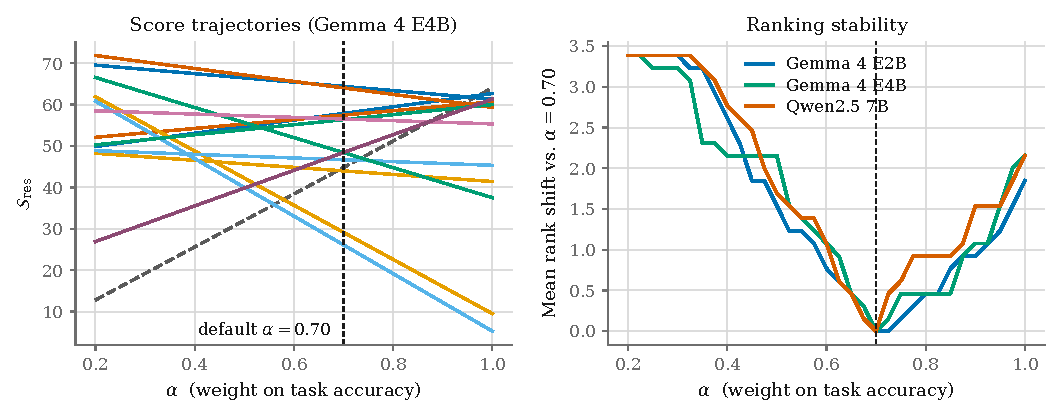
\includegraphics[width=\textwidth]{figures/fig9_alpha_sensitivity.pdf}
\caption{\textbf{The default weight is not load-bearing.} Score trajectories
and mean rank displacement relative to $\alpha = 0.70$.}
\label{fig:alpha}
\end{figure*}

\section{Per-Task, Per-Context and Per-Operating-Point Detail}
\label{app:detail}

\begin{table}[htbp]
\centering
\small
\setlength{\tabcolsep}{2.6pt}
\caption{\textbf{The disagreement between axes is invisible unless the axes
are measured on the same query.} ``Anchor'' means an uncompressed run of the
\emph{same} model is reported; ``paired'' means that run is on the
\emph{same} query. $\triangle$ = sometimes, inconsistently. Discussed in
\S\ref{sec:related}.}
\label{tab:paradigms}
\begin{tabular}{@{}lccccc@{}}
\toprule
\textbf{Practice} & \textbf{Qual.} & \textbf{Mem.} & \textbf{Lat.} & \textbf{Anch.} & \textbf{Pair} \\
\midrule
Long-context suites & \cmark & \xmark & \xmark & \xmark & \xmark \\
Synthetic probes (NIAH, RULER) & \cmark & \xmark & \xmark & \xmark & \xmark \\
Serving-system profilers & \xmark & \cmark & \cmark & \xmark & \xmark \\
Compression method papers & \cmark & $\triangle$ & $\triangle$ & $\triangle$ & \xmark \\
Quality + systems benchmarks & \cmark & \cmark & \cmark & $\triangle$ & \xmark \\
\textbf{This work} & \cmark & \cmark & \cmark & \cmark & \cmark \\
\bottomrule
\end{tabular}
\end{table}

Figure~\ref{fig:heatmap} resolves accuracy by task and
Figure~\ref{fig:context} by context length; both are discussed in
\S\ref{sec:res_tasks}. Figure~\ref{fig:part1} gives the Part~1 ordering at
every operating point and Figure~\ref{fig:pareto} the quality--memory frontier
computed within each model. We compute the frontier per model rather than
pooling: accuracy differences between a 2B and a 7B model reflect base-model
capability, and a frontier drawn across them would be an artefact. The
frontiers are short --- on Gemma~4 E2B a single $4$-bit configuration
dominates everything else, matching dense accuracy at roughly a quarter of the
bits --- which is itself informative about how much headroom remains at these
scales.


\begin{figure}[htbp]
\centering
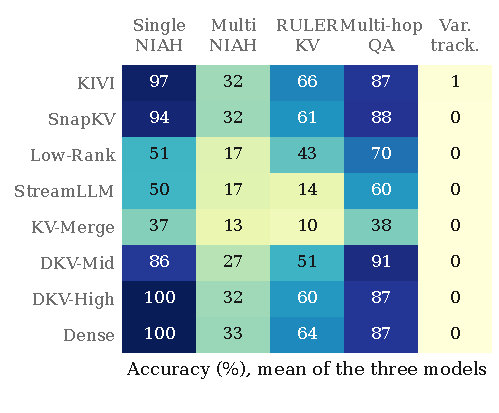
\includegraphics[width=\columnwidth]{figures/fig5_task_heatmap.pdf}
\caption{\textbf{One of our five tasks measures the base model, not the
representation.} Accuracy by task, averaged over the three models and both
budget levels. Variable tracking is at zero for every method \emph{and} for
the uncompressed dense reference, which identifies it as a base-model
limitation rather than a compression failure; without a paired dense run it
would read as a compression result.}
\label{fig:heatmap}
\end{figure}

\begin{figure}[htbp]
\centering
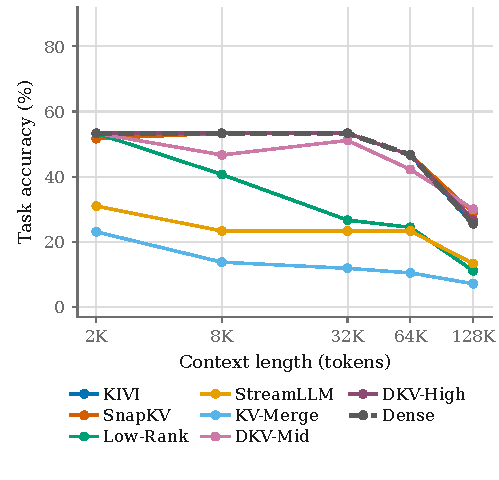
\includegraphics[width=\columnwidth]{figures/fig6_context_scaling.pdf}
\caption{\textbf{The cliff beyond $64$K belongs to the model, not to
compression.} The $2$K--$128$K ladder on Gemma~4 E2B. The dense reference
(dashed) degrades together with the compressed methods, so the drop cannot be
charged to the representation.}
\label{fig:context}
\end{figure}

\begin{figure*}[htbp]
\centering
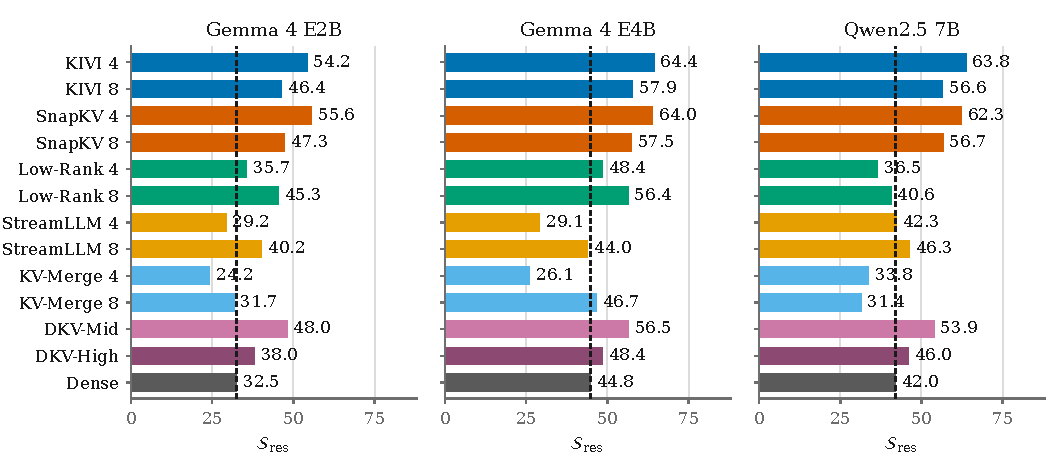
\includegraphics[width=\textwidth]{figures/fig7_part1.pdf}
\caption{\textbf{Representation utility $\Sres$ at every operating point,}
with the dense reference marked (dashed). Dense is not last: at
$\alpha = 0.70$, a method that gives up a few accuracy points for a large
memory saving outscores it.}
\label{fig:part1}
\end{figure*}

\begin{figure*}[htbp]
\centering
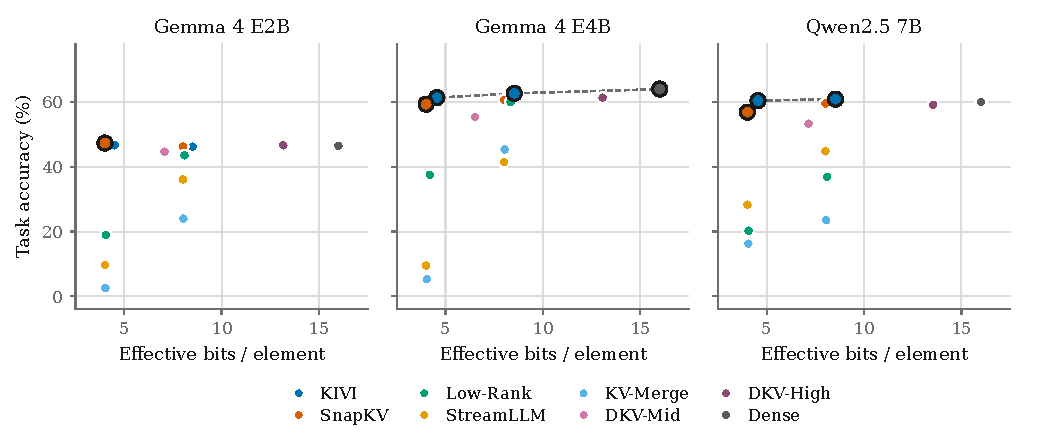
\includegraphics[width=\textwidth]{figures/fig8_pareto.pdf}
\caption{\textbf{Quality--memory frontier, computed within each model.}
Effective bits include metadata. Outlined markers are non-dominated. Frontiers
are not drawn across models, because accuracy differences between models
reflect base-model capability rather than the representation.}
\label{fig:pareto}
\end{figure*}

\section{Measurement Protocol}
\label{app:protocol}

\paragraph{Execution.} Prefill is executed in $4{,}096$-token chunks. The
context transform is applied to the resident PyTorch KV cache after prefill
(or streaming during prefill, for the quantiser), and generation proceeds from
the transformed cache. Decoding is greedy. TTFT is measured with device
synchronisation around the full prefill-plus-transform-plus-first-token path,
so transform cost is charged to the method that incurs it. Peak device memory
is the maximum allocated over the whole query.

\paragraph{Determinism.} Because the dense reference is re-executed in each of
the two budget sweeps, every query carries a free replication of its own
baseline. On Gemma~4 E4B and Qwen2.5~7B all $150$ re-executions produced
byte-identical output text. On Gemma~4 E2B, $64/75$ produced identical text
and exactly one query changed score --- a multi-needle prompt at $128$K.
Run-to-run variance is therefore negligible at the resolution of our claims,
and is smallest on the two models where the matched-pair evidence is
strongest.

\paragraph{Aggregation.} Task quality aggregates as the arithmetic mean of
$Q_{\text{abs}}$ over queries. Memory aggregates by bytes rather than by
query, $\bar{R}_{\text{mem}} = 100\,(1 - \sum_i M_{i,\text{method}} /
\sum_i M_{i,\text{dense}})$, so that the long contexts where compression
matters are not diluted by short ones. A query that failed to complete is
charged the dense footprint and scores zero rather than being dropped, and is
additionally visible in the separately reported coverage $C$.

\paragraph{What is charged to metadata.} Quantisation scales and zero points;
SVD factor matrices; anchor and basis state for the factorised
representations; 32-bit token position indices for eviction methods; and
dtype-alignment padding where the scheme requires it. Partial groups that
cannot be quantised at the target width are charged at 16 bits.

\section{Artifact Appendix}
\label{app:artifact}

\paragraph{Scope.} The artifact reproduces every table, statistic and figure
in this paper from the released per-query records. It does \emph{not} require
re-executing the study: the $3{,}150$ paired executions took approximately
three GPU-days on the machine described in \S\ref{sec:setup}, and the raw
records are shipped so that the analysis is reproducible in minutes on a
CPU-only machine.

\paragraph{Contents.} (i) The harness, including the adapter interface and the
reference implementations noted as ``harness'' in
Table~\ref{tab:provenance}; (ii) the per-query records for all three models,
one JSON line per execution, carrying the task score, analytic footprint,
TTFT, decode throughput and peak device memory for both the dense and the
compressed run; (iii) four analysis scripts.

\paragraph{Reproduction.} The scripts regenerate, in order, every number in
the tables (\texttt{build\_\allowbreak tables.py}), every statistic quoted in
\S\ref{sec:results} (\texttt{decoupling\_\allowbreak analysis.py}) and every
figure (\texttt{make\_\allowbreak figures.py}), reading only the released
records. A fourth script, \texttt{verify\_\allowbreak claims.py}, re-derives
each quantity quoted in the
prose from those outputs and asserts that the manuscript source contains the
matching value; it exits non-zero on any drift. No number in this paper is
transcribed by hand.

\paragraph{Re-executing the study.} Re-running the measurements requires a
CUDA GPU with at least $12$\,GB of device memory and access to the three
open-weight checkpoints named in \S\ref{sec:setup}. Absolute latencies will
differ on other hardware; the paired ratios are the quantities intended to be
comparable.

\typeout{MAINBODYENDS=\pageref{bodyend}}
\end{document}
